\documentclass[11pt,letterpaper]{article}

\usepackage[utf8]{inputenc}
\usepackage[T1]{fontenc}
\usepackage[spanish,es-nodecimaldot,es-tabla]{babel}
\usepackage{lmodern}
\usepackage[margin=2.5cm]{geometry}
\usepackage{amsmath,amssymb}
\usepackage{graphicx}
\usepackage{booktabs}
\usepackage{tabularx}
\usepackage{array}
\usepackage{xcolor}
\usepackage{caption}
\usepackage{subcaption}
\usepackage{enumitem}
\usepackage{listings}
\usepackage{float}
\usepackage[hidelinks]{hyperref}

\definecolor{TecBlue}{RGB}{0,57,166}
\graphicspath{{../figures/}{./}}
\captionsetup{font=small,labelfont=bf}
\setlist{itemsep=2pt,topsep=4pt}
\newcolumntype{L}{>{\raggedright\arraybackslash}X}
\newcolumntype{R}{>{\raggedleft\arraybackslash}X}

\lstset{
  language=Python, basicstyle=\ttfamily\footnotesize, columns=fullflexible,
  keywordstyle=\color{TecBlue}\bfseries, commentstyle=\color{gray}\itshape,
  stringstyle=\color{teal!70!black}, frame=single, rulecolor=\color{gray!40},
  breaklines=true, showstringspaces=false, xleftmargin=4pt, xrightmargin=4pt,
  literate={á}{{\'a}}1 {é}{{\'e}}1 {í}{{\'i}}1 {ó}{{\'o}}1 {ú}{{\'u}}1
           {Á}{{\'A}}1 {É}{{\'E}}1 {Í}{{\'I}}1 {Ó}{{\'O}}1 {Ú}{{\'U}}1
           {ñ}{{\~n}}1 {Ñ}{{\~N}}1 {α}{{$\alpha$}}1
}

\begin{document}

% ---------------------------------------------------------------- Portada
\begin{titlepage}
  \centering
  \IfFileExists{LOGOTEC.png}{\includegraphics[width=0.38\textwidth]{LOGOTEC.png}\par\vspace{1cm}}{\vspace*{2cm}}
  {\Large Tecnológico de Monterrey\par}
  {\large Campus Guadalajara\par}
  \vspace{2.2cm}
  {\color{TecBlue}\Huge\bfseries Monitoreo de Saldo de Inventarios\par}
  \vspace{0.4cm}
  {\Large FEMSA Salud Chile (FCV)\par}
  \vspace{0.8cm}
  {\large Entregable 3: Cadenas de Markov sobre las alertas de inventario\par}
  \vspace{2cm}
  {\large\bfseries Integrantes:\par}
  \vspace{0.3cm}
  {\large
  Rafael Santamaría Heredia | A01646667\par
  Grethel Hernández Olivares | A01640912\par
  Matías Alfredo Hidalgo Guzmán | A01641323\par
  Daniel Rodríguez Peralta | A01646867\par}
  \vspace{1.2cm}
  {\large\bfseries Profesor:\par}
  {\large [Nombre del profesor] --- MA2004B (Gpo [X])\par}
  \vfill
  {\large 25 de noviembre de 2026\par}
\end{titlepage}

\tableofcontents
\newpage

% ---------------------------------------------------------------- Introducción
\section{Introducción}

En los entregables anteriores automatizamos las reglas de auditoría del inventario de FCV: conciliación del Kardex contra la cuenta de existencias, variación mensual del saldo y alertas por partida (semáforo de antigüedad, riesgo por política de canje, estado general y calidad de datos), y las presentamos en un tablero de Power BI. Esas reglas describen \emph{cómo está} el inventario cada mes.

Este entregable agrega la parte predictiva: estimar \emph{hacia dónde va}. Cada alerta de un SKU es un estado que cambia de un mes al siguiente; con los siete meses disponibles (enero a julio de 2026) estimamos una cadena de Markov de primer orden por alerta, estudiamos sus propiedades y la usamos para proyectar qué parte del inventario que hoy está en buen estado terminará estancada. Los resultados se pueden consultar para cualquier SKU en una aplicación de Streamlit.

Todo el código está en el repositorio del equipo:
\begin{itemize}
  \item \texttt{src/reto\_ma2004b/markov.py}: estimación, propiedades, predicción y validación (módulo nuevo, con pruebas en \texttt{tests/test\_markov.py}).
  \item \texttt{app/streamlit\_app.py}: la interfaz.
  \item \texttt{notebooks/03\_cadenas\_markov.ipynb}: el análisis de este reporte.
\end{itemize}

% ---------------------------------------------------------------- Estimación
\section{Cómo estimamos las cadenas}

\subsection{Datos y estados}

Partimos de la tabla completa que genera el pipeline del entregable 2 (\texttt{partidas.csv}): una fila por SKU y mes, 107,302 filas de 16,916 SKU distintos. De ellos, 13,788 aparecen los siete meses y el resto entra o sale del inventario a mitad del periodo. Para cada SKU la secuencia de estados se ve como la tabla de ejemplo del entregable (cuadro~\ref{tab:secuencia}).

\begin{table}[H]
\centering\footnotesize\setlength{\tabcolsep}{3.5pt}
\begin{tabular}{@{}lllllll@{}}
\toprule
Mes & Semáforo (días) & Semáforo (meses) & Riesgo política & Estado general & Rango antigüedad & Conversión \\
\midrule
Ene 2026 & VERDE & VERDE & NORMAL & OK & 31--90 días & OK \\
Feb 2026 & VERDE & VERDE & NORMAL & OK & 31--90 días & OK \\
Mar 2026 & ÁMBAR & VERDE & REVISIÓN & OK & 91--180 días & OK \\
Abr 2026 & ÁMBAR & VERDE & REVISIÓN & OK & 91--180 días & OK \\
May 2026 & ROJO & VERDE & REVISIÓN & OK & 181--365 días & OK \\
Jun 2026 & VERDE & VERDE & NORMAL & OK & 0--30 días & OK \\
Jul 2026 & VERDE & VERDE & NORMAL & OK & 0--30 días & OK \\
\bottomrule
\end{tabular}
\caption{Secuencia de alertas del \texttt{SKU\_002583} (Farmacia, con canje). Recorre el ciclo completo: envejece hasta rojo y vuelve a verde cuando se resurte.}
\label{tab:secuencia}
\end{table}

Modelamos seis alertas, cada una con su propio espacio de estados:

\begin{table}[H]
\centering\small
\begin{tabularx}{\textwidth}{@{}l L l@{}}
\toprule
Alerta & Estados & Estado crítico \\
\midrule
Semáforo de antigüedad en días (hoja de criterios) & VERDE (0--90 días), ÁMBAR (91--180), ROJO ($>$180) & ROJO \\
Semáforo en meses (fórmulas del Kardex) & VERDE ($\le$6 meses), ÁMBAR (7--12), ROJO ($>$12) & ROJO \\
Riesgo por política de canje & NORMAL, REVISIÓN, RIESGO ALTO (rojo sin canje) & RIESGO ALTO \\
Estado general de la partida & OK, MONITOREAR, REVISAR & REVISAR \\
Rango de antigüedad & 0--30, 31--90, 91--180, 181--365, más de 365 días & más de 365 \\
Unidad de conversión & OK, REVISAR, INVÁLIDA & REVISAR \\
\bottomrule
\end{tabularx}
\caption{Alertas modeladas.}
\end{table}

Las alertas de stock, costo y duplicados no se modelaron porque son constantes (todas las partidas están en \texttt{OK}, salvo dos con stock cero); una cadena con un solo estado no aporta información.

Un detalle de los datos guía toda la interpretación: la antigüedad se calcula con \texttt{FULCOM}, que es la fecha de la \emph{última} compra. Cada vez que un producto se resurte, su antigüedad vuelve a cero. Por eso un producto puede regresar de rojo a verde, y por eso las cadenas resultan irreducibles.

\subsection{Estimador}

Para una alerta con estados $\{1,\dots,s\}$ contamos $n_{ij}$, el número de veces que un SKU estaba en el estado $i$ un mes y en el estado $j$ el mes siguiente, sumando sobre todos los SKU y todos los pares de meses consecutivos. Si la cadena es homogénea, el estimador de máxima verosimilitud de la probabilidad de transición es
\begin{equation}
  \hat p_{ij} = \frac{n_{ij}}{n_i}, \qquad n_i = \sum_{k=1}^{s} n_{ik}.
\end{equation}

Tomamos tres decisiones sobre qué transiciones cuentan:

\begin{enumerate}
  \item \textbf{Solo meses consecutivos.} Si un SKU falta un mes, no se cuenta una transición que salte ese mes. Opcionalmente se agrega un estado \texttt{SIN INVENTARIO} para modelar las altas y bajas de productos.
  \item \textbf{Exclusión de fechas sospechosas.} En junio de 2026, 591 SKU tienen una fecha de compra que retrocede exactamente un año respecto a mayo (posible error de captura, ya reportado a FEMSA), y 308 la conservan en julio. Esas partidas pasarían de verde a rojo en un mes, algo físicamente imposible (envejecer 180 días en 30). Excluimos las 1,171 transiciones en las que el origen o el destino tienen esa marca. En la sección~\ref{sec:sensibilidad} se muestra el efecto.
  \item \textbf{Conteo por SKU o por valor.} Por defecto cada transición pesa 1. Con la opción de ponderar, cada transición pesa el valor del inventario del SKU en CLP, lo que da la dinámica del dinero en lugar de la de los productos.
\end{enumerate}

Con estas reglas quedan 89,077 transiciones de 16,307 SKU. El cuadro~\ref{tab:conteos} muestra los conteos y la matriz estimada del semáforo en días.

\begin{table}[H]
\centering\small
\begin{tabular}{@{}l rrr c rrr@{}}
\toprule
 & \multicolumn{3}{c}{Conteos $n_{ij}$} & & \multicolumn{3}{c}{Probabilidades $\hat p_{ij}$} \\
\cmidrule{2-4}\cmidrule{6-8}
Mes actual $\backslash$ siguiente & VERDE & ÁMBAR & ROJO & & VERDE & ÁMBAR & ROJO \\
\midrule
VERDE & 62,262 & 1,850 & 0 & & 0.971 & 0.029 & 0.000 \\
ÁMBAR & 524 & 3,199 & 1,118 & & 0.108 & 0.661 & 0.231 \\
ROJO & 255 & 0 & 19,869 & & 0.013 & 0.000 & 0.987 \\
\bottomrule
\end{tabular}
\caption{Semáforo de antigüedad en días: transiciones observadas y matriz de transición estimada (enero a julio de 2026).}
\label{tab:conteos}
\end{table}

\subsection{Matriz de un SKU: suavizado hacia la matriz global}

El entregable pide poder estimar la matriz para cualquier SKU. Con siete meses, un SKU tiene como máximo seis transiciones, así que su matriz de máxima verosimilitud casi siempre tiene renglones vacíos (estados que nunca visitó) o probabilidades de 0 y 1 poco creíbles. Por ejemplo, el \texttt{SKU\_002583} solo pasó una vez por rojo y salió de ahí, de modo que su estimación propia da $\hat p_{\text{ROJO},\text{VERDE}} = 1$.

Para evitarlo usamos el estimador bayesiano con una previa de Dirichlet centrada en la matriz global $q$:
\begin{equation}
  \hat p^{(\text{sku})}_{ij} = \frac{n_{ij} + \alpha\, q_{ij}}{n_i + \alpha}.
\end{equation}
El parámetro $\alpha$ se interpreta como cuántas transiciones de la población vale la previa: con $\alpha = 0$ se usa solo la historia del SKU, con $\alpha$ grande la estimación se acerca a la global, y un estado que el SKU nunca visitó hereda el renglón global. Usamos $\alpha = 2$ por defecto; en la app se puede mover. La figura~\ref{fig:sku} compara ambas estimaciones.

\begin{figure}[H]
\centering
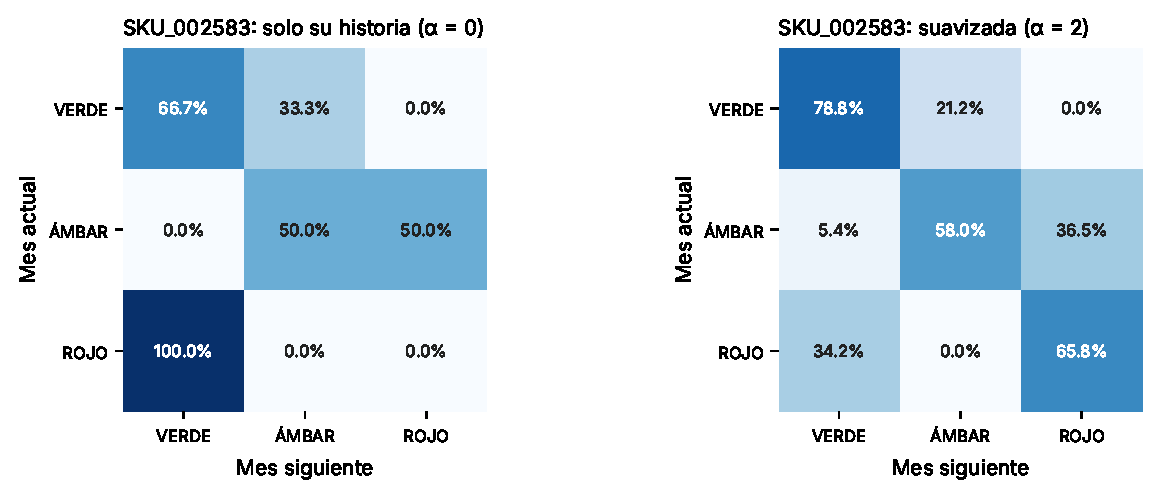
\includegraphics[width=0.85\textwidth]{markov_sku_ejemplo.pdf}
\caption{Matriz del \texttt{SKU\_002583}: con su historia sola (seis transiciones) y suavizada hacia la global con $\alpha = 2$.}
\label{fig:sku}
\end{figure}

\subsection{Código modular}

El módulo \texttt{markov.py} expone funciones que sirven para cualquier alerta, SKU o segmento:

\begin{lstlisting}
from reto_ma2004b import markov as M

r = M.estimar(partidas, "SEMAFORO_DIAS")                          # todo el inventario
r = M.estimar(partidas, "SEMAFORO_DIAS", filtros={"POLITICA_CANJE": "P0"})   # un segmento
r = M.estimar(partidas, "SEMAFORO_DIAS", codigo="SKU_002583", alfa=2)       # un SKU
todas = M.estimar_sku(partidas, "SKU_002583")                     # las 6 alertas de un SKU

M.propiedades(r.matriz)        # clases, periodo, ergodicidad, estacionaria, absorbentes
M.tiempos_primer_paso(r.matriz, "ROJO")
M.proyectar(r.matriz, distribucion_inicial, pasos=3)
M.riesgo_por_sku(partidas, "SEMAFORO_DIAS", pasos=3)              # lista de trabajo
M.prueba_homogeneidad(partidas, "SEMAFORO_DIAS")
M.backtest(partidas, "SEMAFORO_DIAS", "2026-04-01")
\end{lstlisting}

Las propiedades se calculan sin depender del tamaño de la matriz: las clases comunicantes se obtienen con la cerradura transitiva del grafo de transiciones (algoritmo de Warshall), el periodo de cada clase como el máximo común divisor de las diferencias de nivel en un recorrido en anchura, y la distribución estacionaria resolviendo $\pi P = \pi$ con $\sum_i \pi_i = 1$. Las pruebas (\texttt{uv run pytest}) verifican cada función con cadenas pequeñas cuyo resultado se conoce a mano: una cadena periódica de periodo 2, una con un estado absorbente, una regular con estacionaria $(5/6, 1/6)$, el suavizado y la exclusión de fechas sospechosas.

% ---------------------------------------------------------------- Propiedades
\section{Propiedades de las cadenas}

\begin{figure}[H]
\centering
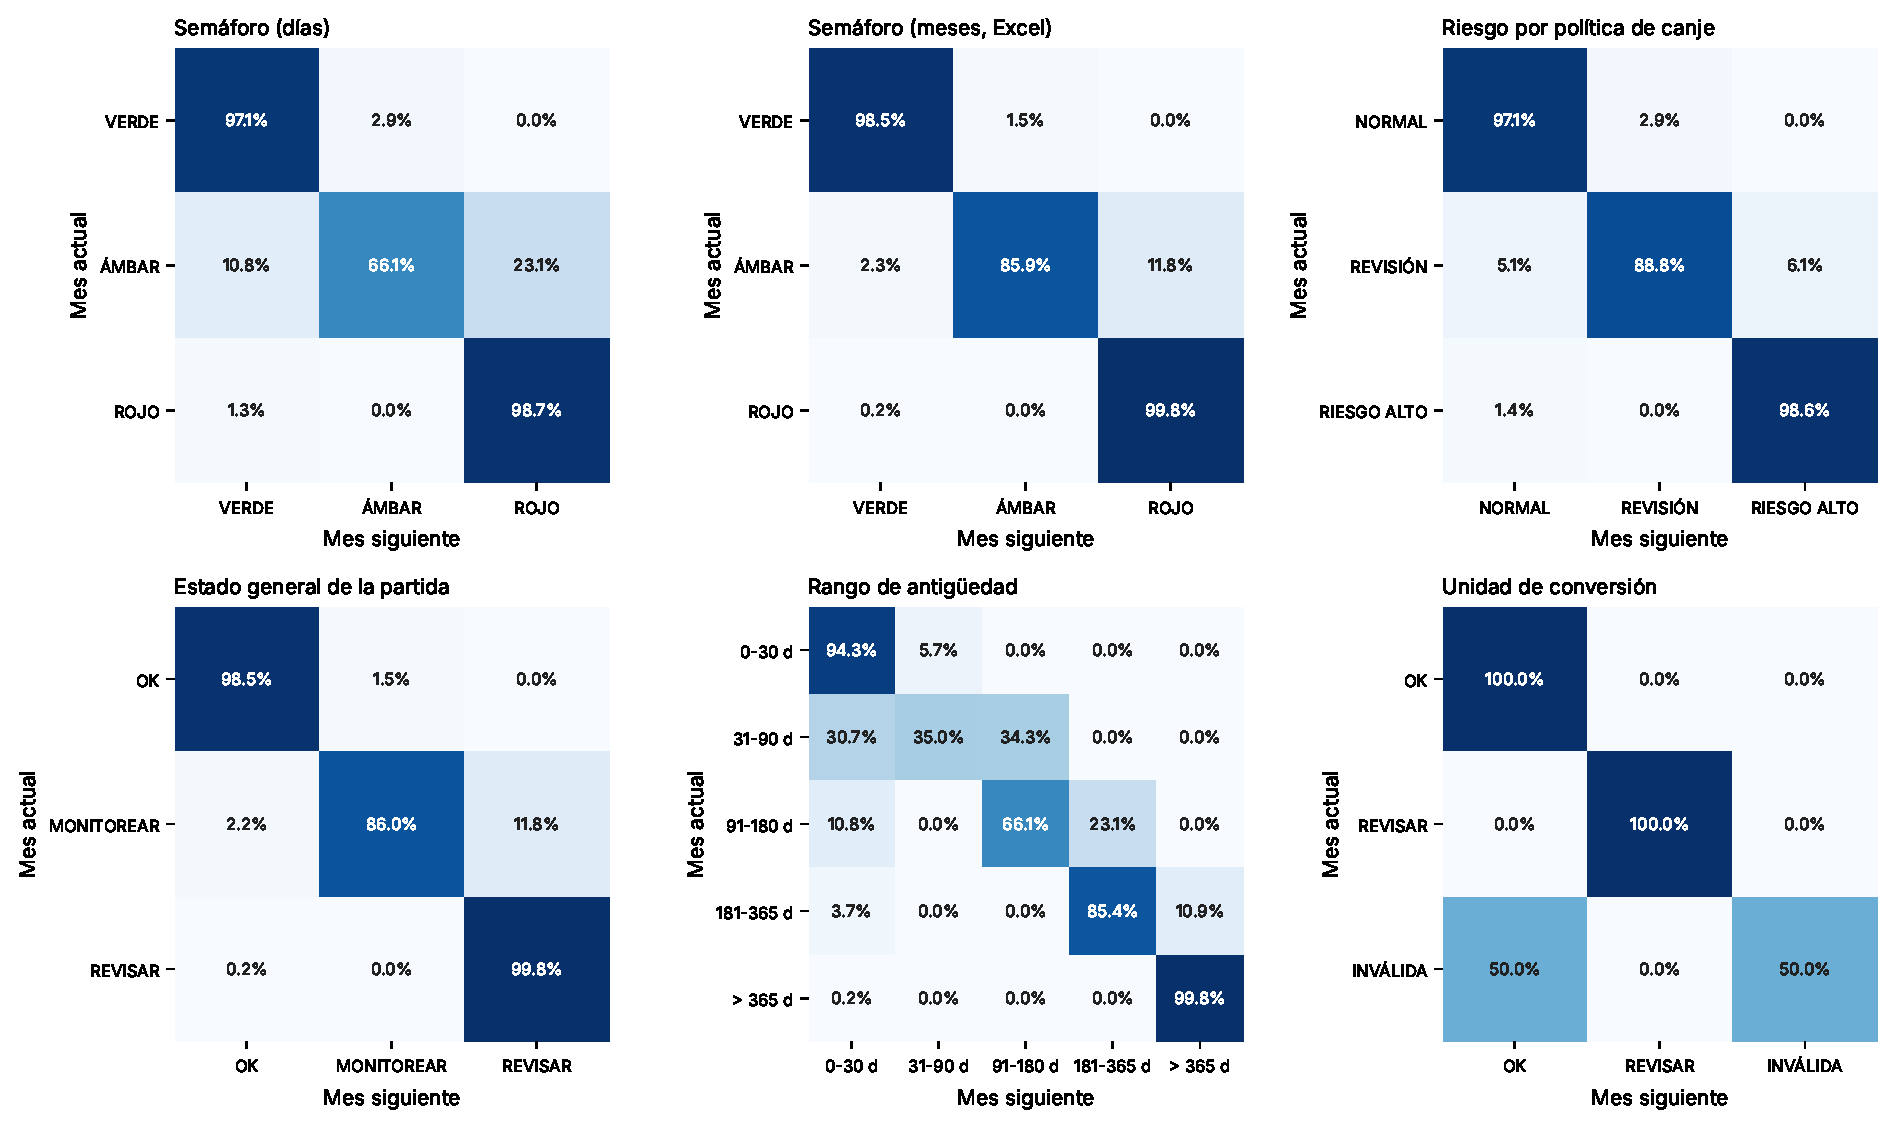
\includegraphics[width=\textwidth]{markov_seis_alertas.pdf}
\caption{Matrices de transición estimadas para las seis alertas (todo el inventario, enero a julio de 2026).}
\label{fig:seis}
\end{figure}

\begin{table}[H]
\centering\small
\begin{tabularx}{\textwidth}{@{}L c c c c r r@{}}
\toprule
Alerta & Clases & Irreducible & Aperiódica & Ergódica & \% hoy en crítico & \% largo plazo \\
\midrule
Semáforo (días) & 1 & Sí & Sí & Sí & 22.8 & 58.8 \\
Semáforo (meses) & 1 & Sí & Sí & Sí & 15.2 & 84.5 \\
Riesgo por política & 1 & Sí & Sí & Sí & 15.0 & 47.1 \\
Estado general & 1 & Sí & Sí & Sí & 15.6 & 84.5 \\
Rango de antigüedad & 1 & Sí & Sí & Sí & 15.8 & 83.6 \\
Unidad de conversión & 2 & No & Sí & No & 0.7 & --- \\
\bottomrule
\end{tabularx}
\caption{Propiedades de las cadenas. ``\% hoy'' es la proporción de SKU en el estado crítico en julio de 2026; ``\% largo plazo'' es su probabilidad en la distribución estacionaria $\pi$.}
\label{tab:propiedades}
\end{table}

\paragraph{Cinco de las seis cadenas son ergódicas.} Son irreducibles porque desde cualquier estado se puede regresar a verde (el resurtido reinicia la antigüedad), y aperiódicas porque todos los estados tienen $p_{ii} > 0$: en una clase irreducible basta un lazo para que el periodo sea 1. Además son regulares (alguna potencia $P^k$ tiene todas sus entradas positivas). En una cadena finita esto garantiza una distribución estacionaria única a la que converge el sistema desde cualquier punto de partida.

\paragraph{La unidad de conversión no lo es.} Tiene dos clases: \{OK, INVÁLIDA\} y \{REVISAR\}, con REVISAR absorbente ($p = 1$) y OK prácticamente absorbente (3 salidas en 88,435 transiciones). Tiene sentido: la unidad de conversión es un atributo del catálogo del producto, no algo que cambie con el tiempo. Para esta alerta Markov no predice nada útil; se resuelve corrigiendo el catálogo.

\paragraph{La estructura del semáforo.} La matriz del cuadro~\ref{tab:conteos} tiene ceros que reflejan cómo funciona la antigüedad. Un producto verde nunca salta directo a rojo (necesita pasar 90 días en ámbar) y un producto rojo nunca regresa a ámbar (si se resurte, vuelve a verde). El ciclo es verde $\to$ ámbar $\to$ rojo $\to$ verde.

\paragraph{El rojo se acumula.} Hoy el 22.8\,\% de los SKU está en rojo, pero el equilibrio de largo plazo es 58.8\,\%. La razón está en la asimetría de la matriz: desde ámbar se entra a rojo con 23\,\% de probabilidad al mes, mientras que desde rojo se sale con solo 1.3\,\%. El cuadro~\ref{tab:tiempos} resume los tiempos esperados.

\begin{table}[H]
\centering\small
\begin{tabular}{@{}l r r r r@{}}
\toprule
Estado & $\pi_i$ & Retorno $1/\pi_i$ (meses) & Meses hasta ROJO & Duración de una visita $1/(1-p_{ii})$ \\
\midrule
VERDE & 0.379 & 2.6 & 55.2 & 34.7 \\
ÁMBAR & 0.032 & 31.0 & 20.6 & 2.9 \\
ROJO & 0.588 & 1.7 & 0 & 78.9 \\
\bottomrule
\end{tabular}
\caption{Distribución estacionaria, tiempo medio de retorno, tiempo medio de primer paso a rojo y duración esperada de una estancia (semáforo en días).}
\label{tab:tiempos}
\end{table}

Un producto verde tarda en promedio 55 meses en llegar a rojo: la mayoría se resurte antes de envejecer. Pero una vez en rojo, la estancia esperada es de casi 79 meses. En la práctica, lo que llega a rojo no sale por sí solo; necesita una acción (canje, promoción o baja). Las cadenas del semáforo en meses y del estado general muestran lo mismo de forma más extrema (99.8\,\% de permanencia en rojo), porque su umbral de rojo es de un año.

% ---------------------------------------------------------------- Resultados
\section{Resultados: predicción y la aplicación}

\subsection{Hacia dónde va el inventario}

La distribución dentro de $k$ meses es $x_{t+k} = x_t\, P^k$. Partiendo de julio de 2026, la figura~\ref{fig:proyeccion} proyecta doce meses, tanto en número de SKU como en valor del inventario (con la matriz ponderada por valor).

\begin{figure}[H]
\centering
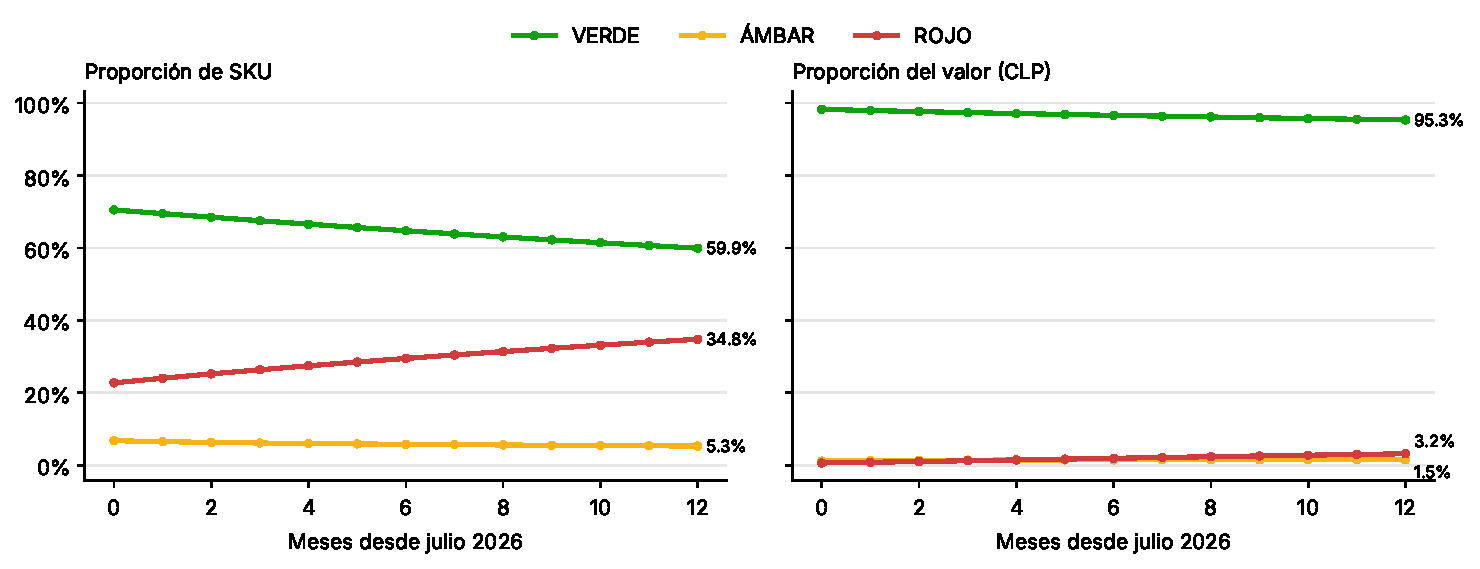
\includegraphics[width=\textwidth]{markov_proyeccion.pdf}
\caption{Proyección de la distribución del semáforo en días a partir de julio de 2026.}
\label{fig:proyeccion}
\end{figure}

Las dos vistas cuentan historias distintas. Por número de SKU, la proporción en rojo pasa de 22.8\,\% a 26.4\,\% en tres meses y a 34.8\,\% en un año. Por valor, el 98\,\% del inventario está en verde y en un año seguiría en 95\,\%: los productos caros rotan rápido y lo que se estanca son, sobre todo, productos de poco valor. Para el riesgo de sobrevaluación, que se mide en pesos, la segunda vista es la relevante. Aun así, el valor que hoy está en verde y estaría en rojo dentro de seis meses es de unos 965 millones de CLP, sobre un inventario de 116,975 millones.

\subsection{Lista de productos en riesgo}

El promedio no dice \emph{qué} productos atender. Para cada SKU que hoy no está en rojo calculamos, con su propia matriz suavizada, la probabilidad de estar en rojo dentro de tres meses, $[P_{\text{sku}}^3]_{\text{actual},\,\text{ROJO}}$, y la multiplicamos por su valor. De los 11,626 SKU evaluados, el valor esperado en rojo dentro de tres meses es de 1,101 millones de CLP. Los primeros lugares son productos ámbar de alto valor, con 91 a 121 días desde su última compra y cerca de 48\,\% de probabilidad de llegar a rojo en tres meses si no se resurten o se mueven (figura~\ref{fig:app-riesgo}). En cambio, un SKU verde tiene en promedio 0.7\,\% de probabilidad.

\subsection{La aplicación de Streamlit}

Elegimos la opción recomendada: una aplicación de Streamlit que lee la tabla procesada (la que genera el pipeline o un CSV que se cargue) y construye automáticamente la matriz para lo que se pida. Se ejecuta con \texttt{uv run streamlit run app/streamlit\_app.py}. En la barra lateral se elige:

\begin{itemize}
  \item la alerta;
  \item el ámbito: todo el inventario, un segmento (línea y política de canje) o un SKU, con el parámetro de suavizado $\alpha$;
  \item si se excluyen las fechas sospechosas, si se incluye el estado \texttt{SIN INVENTARIO}, si se pondera por valor y el horizonte de predicción.
\end{itemize}

Tiene cinco pestañas: la matriz de transición (con la secuencia observada del SKU, los conteos y la descarga en CSV), las propiedades de la cadena, la predicción, la lista de riesgo y la validación del modelo.

\begin{figure}[H]
\centering
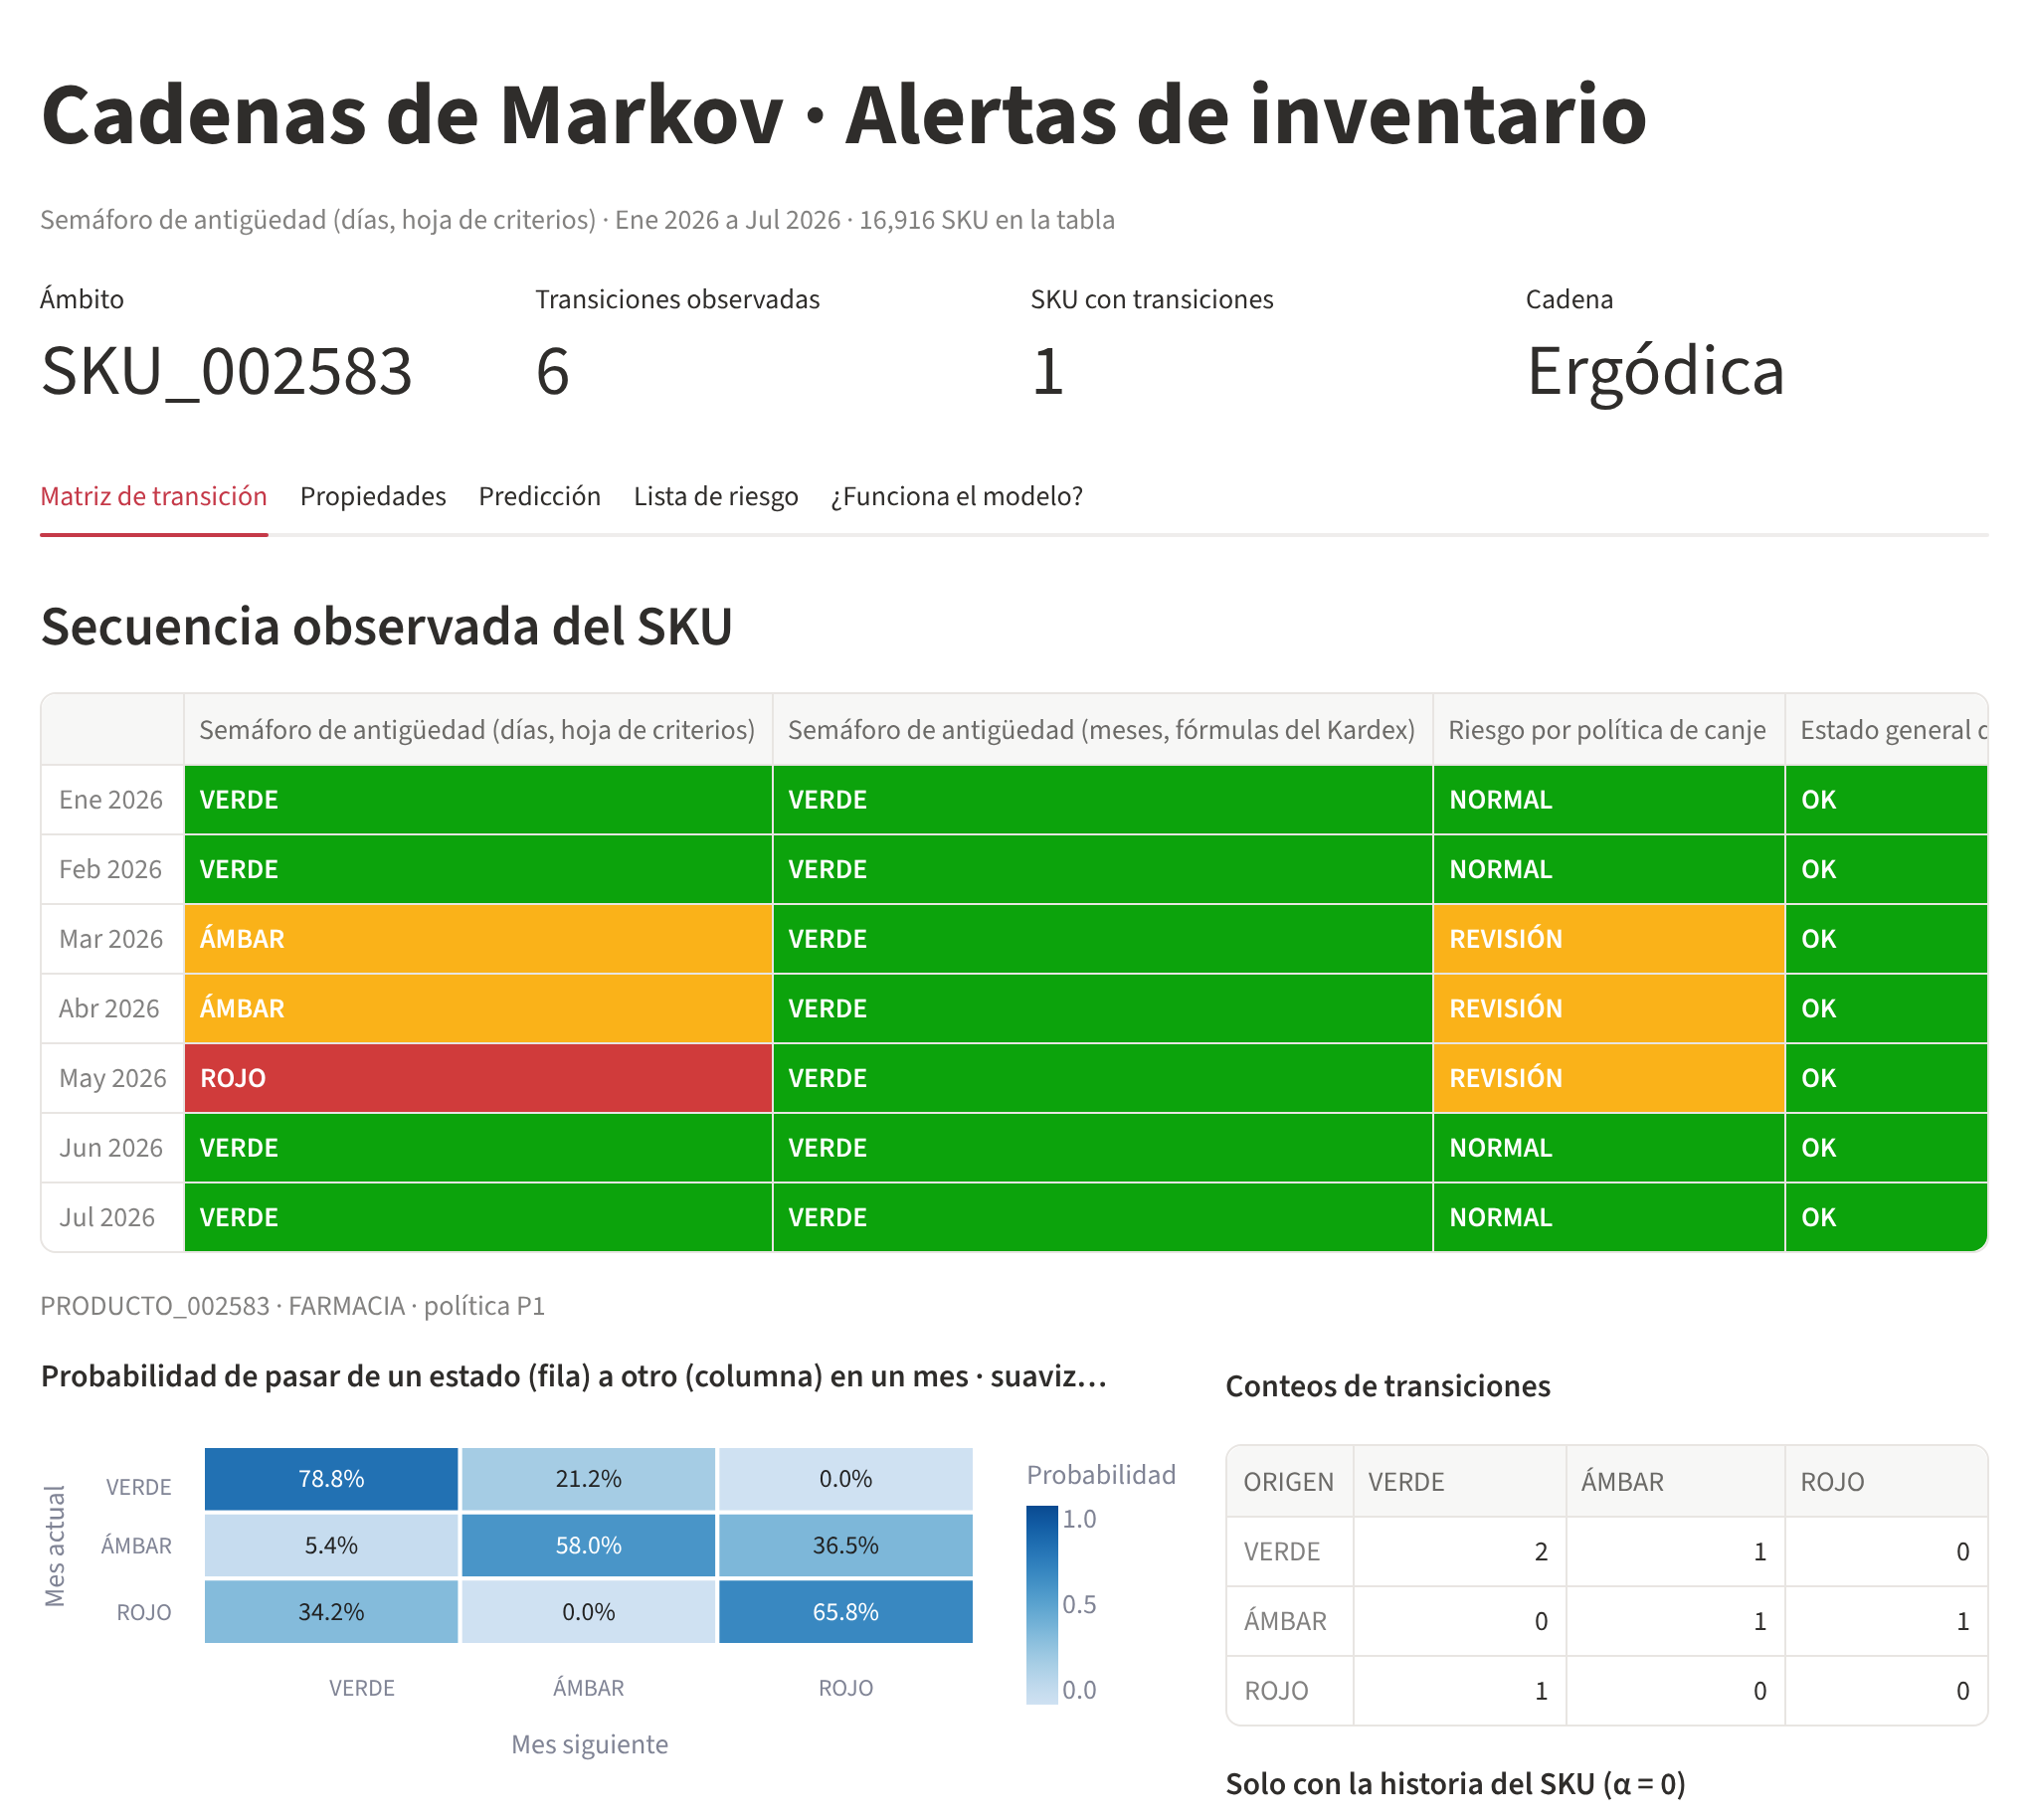
\includegraphics[width=0.92\textwidth]{app_sku.png}
\caption{Aplicación: matriz de un SKU. Arriba, la secuencia observada de las seis alertas; abajo, la matriz suavizada y los conteos.}
\label{fig:app-sku}
\end{figure}

\begin{figure}[H]
\centering
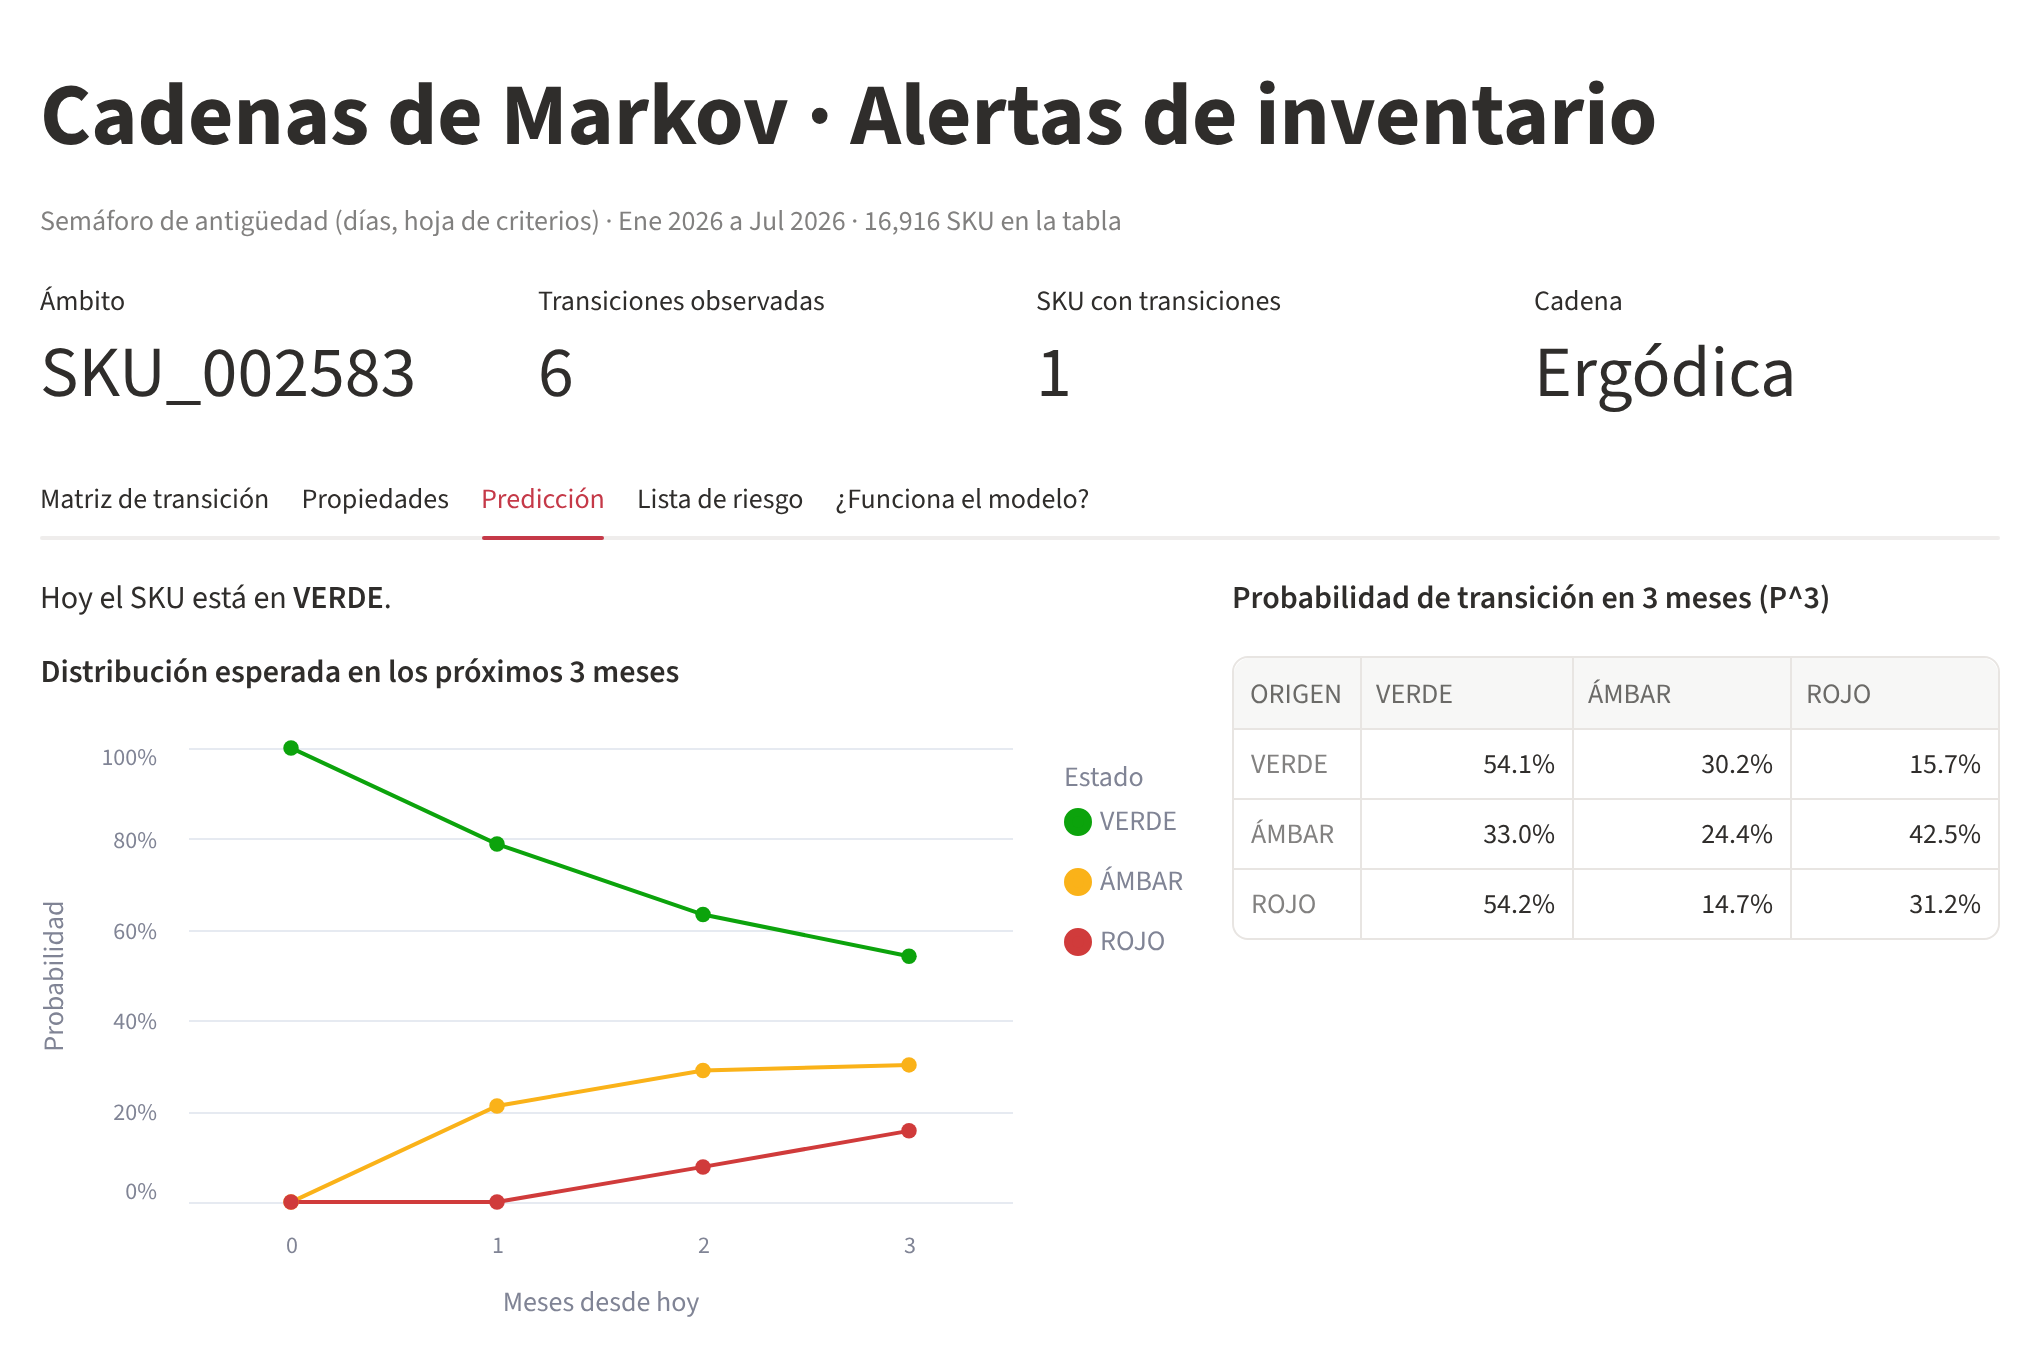
\includegraphics[width=0.8\textwidth]{app_sku_pred.png}
\caption{Aplicación: predicción para el \texttt{SKU\_002583}. Hoy está en verde y su probabilidad de estar en rojo en tres meses es 15.7\,\%, muy por encima del 1.7\,\% promedio, porque en su historia ya hizo el ciclo completo.}
\label{fig:app-pred}
\end{figure}

\begin{figure}[H]
\centering
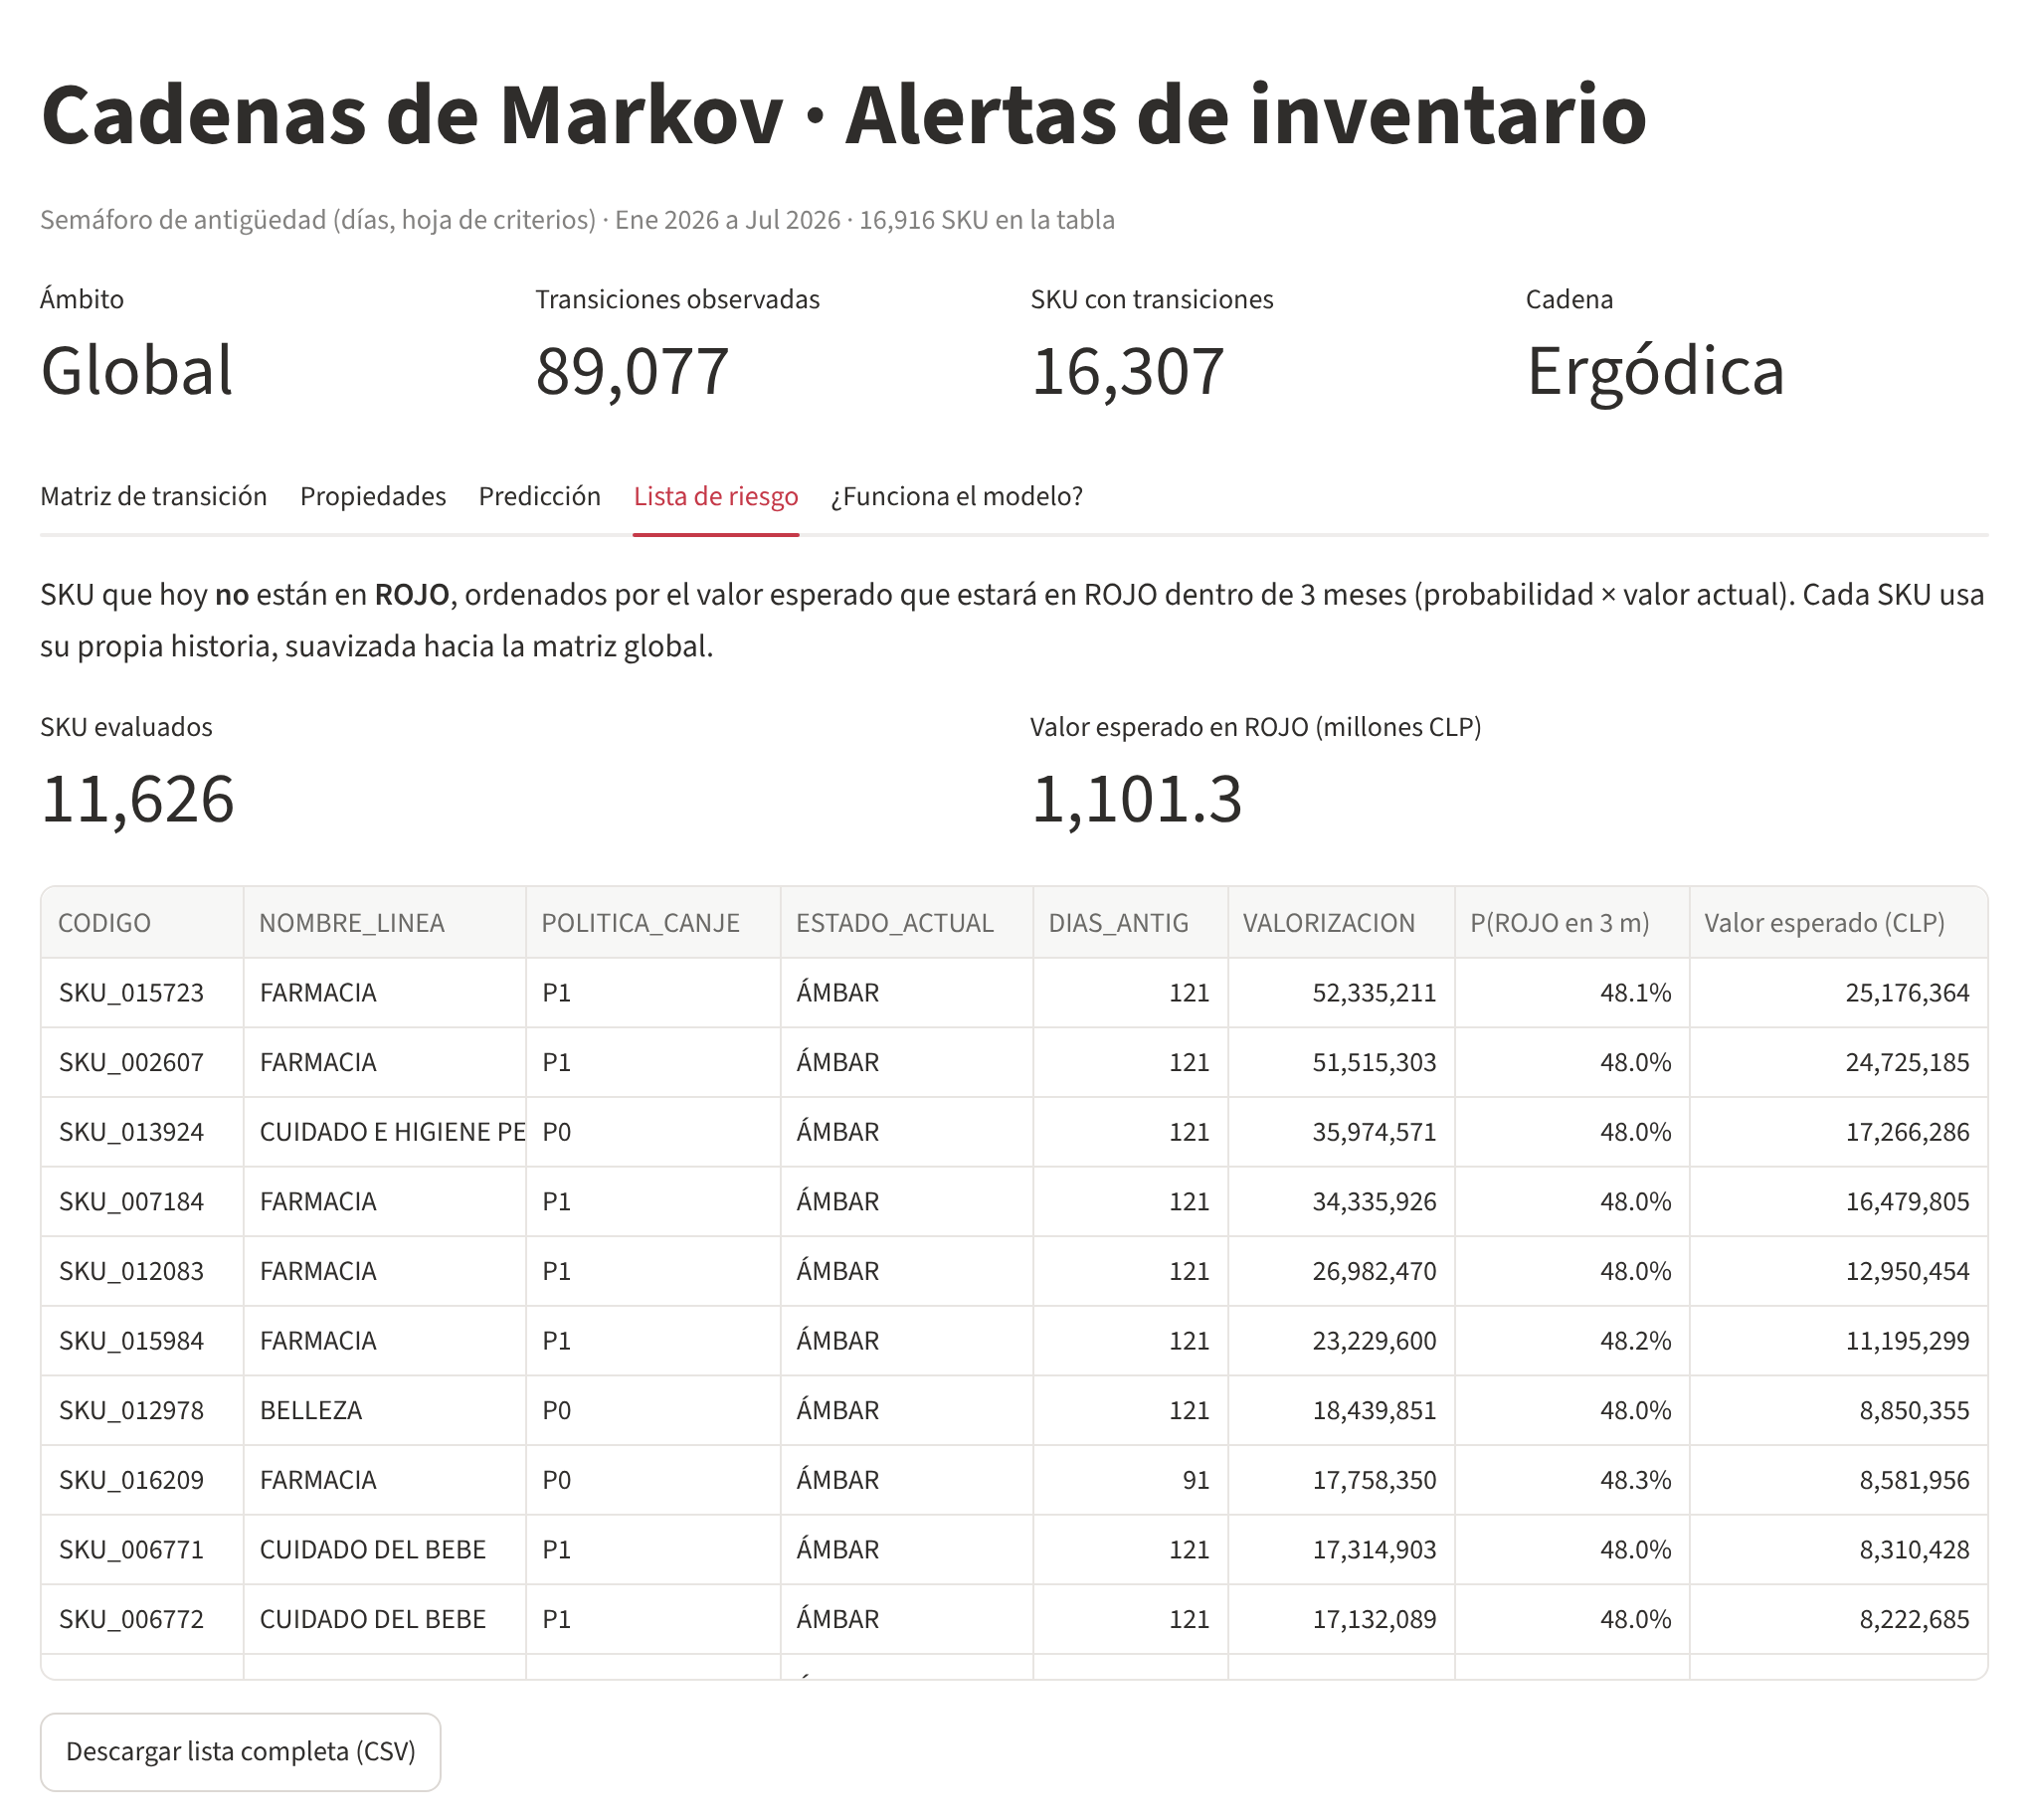
\includegraphics[width=0.8\textwidth]{app_riesgo.png}
\caption{Aplicación: SKU que hoy no están en rojo, ordenados por el valor esperado que estará en rojo dentro de tres meses.}
\label{fig:app-riesgo}
\end{figure}

En Power BI, la página \emph{Transiciones} del tablero ya muestra la matriz agregada de los rangos de antigüedad por mes. La matriz por SKU quedó en Streamlit porque requiere recalcular el suavizado y las potencias de la matriz al vuelo, algo que el modelo de Power BI no hace de forma natural.

% ---------------------------------------------------------------- Validación
\section{¿Se sostiene el supuesto de Markov?}
\label{sec:validacion}

\paragraph{Homogeneidad.} El modelo supone que la matriz es la misma todos los meses. Lo probamos con la prueba de razón de verosimilitud de Anderson y Goodman, que compara la matriz de cada par de meses con la matriz conjunta:
\[
  G = 2 \sum_t \sum_{i,j} n_{ij}(t) \ln\frac{\hat p_{ij}(t)}{\hat p_{ij}} \;\sim\; \chi^2_{gl}.
\]
Para el semáforo en días, $G = 3{,}776.5$ con 20 grados de libertad ($p < 10^{-10}$): \textbf{se rechaza la homogeneidad}. La figura~\ref{fig:homog} muestra dónde está el problema. Verde y rojo son estables mes a mes, pero el ámbar no: la probabilidad de pasar de ámbar a rojo va de 0.3\,\% a 63\,\% según el mes. La causa es de calendario. El ámbar es una ventana de 90 días y lo que pase con él depende de cuándo se compraron los productos que están ahí; cuando un lote grande se compró el mismo día, todo el lote cruza a rojo en el mismo mes.

\begin{figure}[H]
\centering
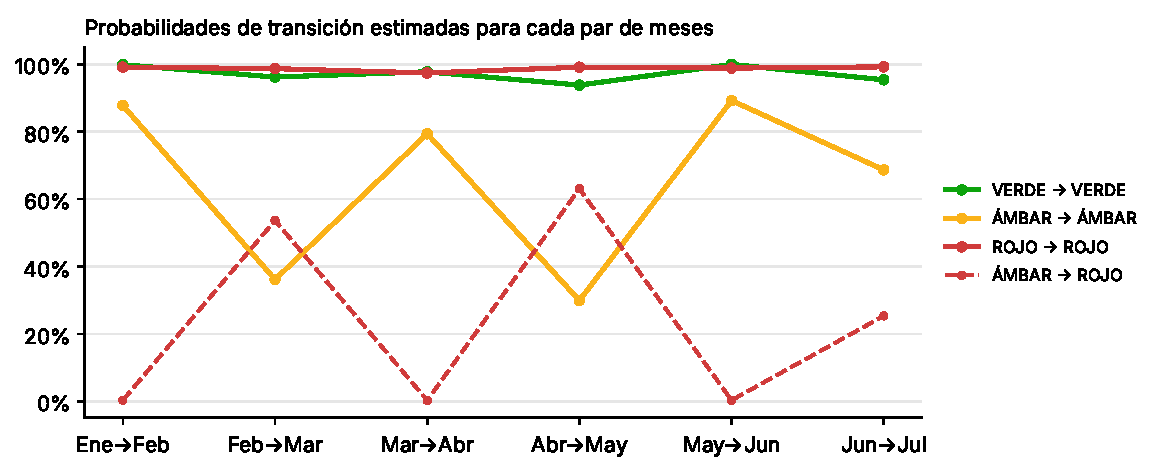
\includegraphics[width=0.85\textwidth]{markov_homogeneidad.pdf}
\caption{Probabilidades de transición estimadas por separado para cada par de meses consecutivos.}
\label{fig:homog}
\end{figure}

\paragraph{Prueba fuera de muestra.} Que la matriz no sea constante no implica que no sirva para predecir. Estimamos la matriz solo con las transiciones de enero a abril, tomamos los SKU de abril y proyectamos su distribución a mayo, junio y julio (figura~\ref{fig:backtest}). El error absoluto medio es de 1.3 puntos porcentuales y el máximo de 2.4: a nivel agregado y para horizontes de uno a tres meses, el modelo funciona. El error se concentra en el ámbar de julio (proyectado 4.9\,\%, observado 7.1\,\%), el estado más sensible al calendario de compras.

\begin{figure}[H]
\centering
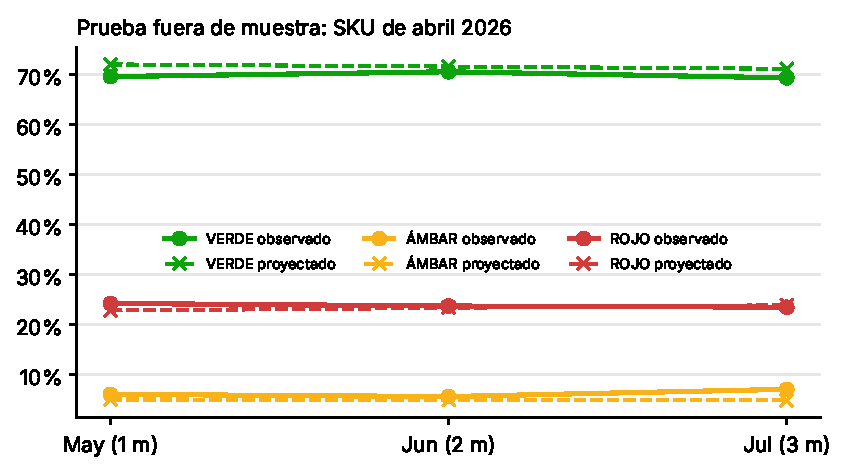
\includegraphics[width=0.75\textwidth]{markov_backtest.pdf}
\caption{Proyección con la matriz estimada hasta abril contra lo observado en los mismos SKU.}
\label{fig:backtest}
\end{figure}

\subsection{Sensibilidad}
\label{sec:sensibilidad}

\paragraph{Fechas sospechosas.} Si no se excluyen, aparece una probabilidad de 0.9\,\% de pasar de verde a rojo en un mes y la salida de rojo se duplica (de 1.3\,\% a 2.6\,\%). Ninguna de las dos es real: son productos cuya fecha de compra retrocedió un año en junio y regresó en julio. Por eso la exclusión está activa por defecto.

\paragraph{Altas y bajas.} Con el estado \texttt{SIN INVENTARIO}, un SKU rojo sale del inventario con 6.2\,\% de probabilidad al mes, contra 0.4\,\% de uno verde: el inventario estancado es el que termina dándose de baja.

\paragraph{Segmentos.} Las matrices por política de canje y por línea difieren de forma útil (cuadro~\ref{tab:segmentos}).

\begin{table}[H]
\centering\footnotesize\setlength{\tabcolsep}{4pt}
\begin{tabular}{@{}l r r r r r r@{}}
\toprule
Segmento & SKU & Verde$\to$Ámbar & Ámbar$\to$Rojo & Rojo$\to$Verde & Rojo hoy & Rojo largo plazo \\
\midrule
Sin canje (P0) & 8,491 & 3.9\,\% & 23.7\,\% & 1.4\,\% & 29.1\,\% & 62.7\,\% \\
Con canje (P1) & 7,816 & 2.0\,\% & 22.0\,\% & 1.0\,\% & 16.0\,\% & 57.0\,\% \\
\midrule
Farmacia & 4,820 & 1.3\,\% & 21.4\,\% & 2.1\,\% & 11.9\,\% & 26.7\,\% \\
Alimentos & 649 & 1.0\,\% & 26.1\,\% & 1.6\,\% & 15.4\,\% & 34.1\,\% \\
Veterinaria & 247 & 0.7\,\% & 17.6\,\% & 0.5\,\% & 27.3\,\% & 45.4\,\% \\
Belleza & 6,544 & 4.6\,\% & 23.4\,\% & 1.5\,\% & 26.3\,\% & 63.6\,\% \\
Cuidado e higiene personal & 2,812 & 3.2\,\% & 23.6\,\% & 0.7\,\% & 25.3\,\% & 75.4\,\% \\
Mercaderías varias & 412 & 3.4\,\% & 19.1\,\% & 0.4\,\% & 70.7\,\% & 79.4\,\% \\
Distribuibles & 175 & 5.1\,\% & 19.6\,\% & 0.7\,\% & 28.4\,\% & 81.9\,\% \\
Cuidado del bebé & 648 & 3.3\,\% & 25.7\,\% & 0.2\,\% & 34.0\,\% & 93.8\,\% \\
\bottomrule
\end{tabular}
\caption{Probabilidades mensuales seleccionadas por segmento (semáforo en días).}
\label{tab:segmentos}
\end{table}

% ---------------------------------------------------------------- Estrategias
\section{Estrategias de negocio sugeridas}

\begin{enumerate}
  \item \textbf{Actuar en ámbar, no en rojo.} La transición ámbar $\to$ rojo (23\,\% al mes) es el punto de no retorno práctico: una vez en rojo, la estancia esperada es de casi siete años. La lista de riesgo identifica los productos ámbar de mayor valor; para ellos conviene decidir antes de los 180 días entre resurtir solo si hay demanda, promover o devolver al proveedor.
  \item \textbf{Priorizar los productos sin canje (P0).} Envejecen casi el doble de rápido (3.9\,\% contra 2.0\,\% de verde a ámbar), hoy tienen casi el doble de SKU en rojo (29\,\% contra 16\,\%) y no se pueden devolver, así que concentran la pérdida potencial. Para ellos el umbral de revisión podría adelantarse a los 90 días.
  \item \textbf{Revisar surtido y compras en las líneas con equilibrio alto en rojo.} En Cuidado del bebé, Distribuibles y Mercaderías varias casi nada sale de rojo; si la dinámica no cambia, la mayor parte de sus SKU terminaría estancada. Son candidatas a reducir profundidad de compra o depurar catálogo.
  \item \textbf{Usar la proyección por valor como provisión.} El valor esperado que llegará a rojo en los próximos meses (unos 1,100 millones de CLP a tres meses en la lista de riesgo) es una base cuantitativa para estimar la reserva por obsolescencia, en lugar de un porcentaje fijo.
  \item \textbf{Depurar el inventario rojo existente.} Con 6\,\% mensual de salida natural y solo 1.3\,\% de regreso a verde, el rojo actual no se va a resolver solo. Conviene una campaña de canje o baja contable controlada, que además reduce el riesgo de sobrevaluación.
  \item \textbf{Corregir los datos antes de modelar.} El error de fechas de junio crea transiciones imposibles y cambia las probabilidades de salida de rojo. Validar que \texttt{FULCOM} no retroceda debería ser un control previo al cierre.
\end{enumerate}

% ---------------------------------------------------------------- Conclusiones
\section{Conclusiones y limitaciones}

Estimamos cadenas de Markov de primer orden para seis alertas con 89,077 transiciones de 16,307 SKU. Cinco cadenas son ergódicas y regulares, con una estructura que refleja cómo funciona la antigüedad: avanza un estado a la vez y se reinicia con cada compra. La sexta (unidad de conversión) es reducible con un estado absorbente, porque describe un atributo fijo. El hallazgo principal es la asimetría entre entrar y salir del rojo, que hace que el equilibrio de largo plazo tenga más del doble de SKU estancados que hoy, aunque en valor el inventario se mantiene mayormente sano. El módulo y la app permiten repetir el análisis para cualquier SKU, segmento o alerta, y la lista de riesgo convierte el modelo en una herramienta de trabajo.

Limitaciones:
\begin{itemize}
  \item \textbf{Historia corta.} Siete meses dan seis transiciones por SKU. Las matrices individuales dependen mucho del suavizado, y las probabilidades pequeñas (como salir de rojo) tienen un intervalo de confianza amplio.
  \item \textbf{No homogeneidad.} La matriz cambia de un mes a otro, sobre todo en ámbar, por el calendario de compras. El modelo homogéneo funciona como promedio a corto plazo, pero las proyecciones a un año deben leerse como tendencia, no como pronóstico puntual. Con más historia se podría estimar una matriz por temporada o modelar la antigüedad exacta en días.
  \item \textbf{Primer orden.} Suponemos que el siguiente estado solo depende del actual. En realidad, dentro de ámbar no es lo mismo tener 95 días que 175; el rango de antigüedad con cinco estados mitiga parte de esto.
  \item \textbf{Datos con errores conocidos.} El error de fechas de junio se excluyó, pero si FEMSA confirma la corrección convendría reprocesar con las fechas correctas.
  \item \textbf{La antigüedad es de la última compra.} El modelo describe cuánto tiempo pasa sin resurtir, no la caducidad real de cada lote. Si el Kardex incluyera lote y fecha de vencimiento, el mismo método se podría aplicar directamente a la caducidad.
\end{itemize}

\end{document}
